\documentclass[12pt, a4paper]{article}
\usepackage{graphicx}
\graphicspath{ {./imgs/} }
\usepackage{float}
\usepackage{listings}
\usepackage{color}
\usepackage{hyperref}

\definecolor{codegreen}{rgb}{0,0.6,0}
\definecolor{codegray}{rgb}{0.5,0.5,0.5}
\definecolor{codeorange}{rgb}{1,0.49,0}
\definecolor{backcolour}{rgb}{0.95,0.95,0.96}

\lstset{
    backgroundcolor=\color{backcolour},       
    commentstyle=\color{codegray},
    keywordstyle=\color{codeorange},
    numberstyle=\tiny\color{codegray},
    stringstyle=\color{codegreen},
    basicstyle=\ttfamily\footnotesize,
    breakatwhitespace=false,         
    breaklines=true,                 
    captionpos=b,                    
    keepspaces=true,                 
    numbers=left,                    
    numbersep=5pt,                  
    showspaces=false,                
    showstringspaces=false,
    showtabs=false,                  
    tabsize=2,
    xleftmargin=10pt,
}
\renewcommand{\lstlistingname}{Code}

\counterwithin{figure}{section}

%to write code:
%\begin{lstlisting}[language=java, caption={my caption}]
%    
%\end{lstlisting}

%to insert an image
%\begin{figure}[H]
%  \centering
%  \includegraphics[width=\columnwidth]{img.png}
%  \caption{description of the image}
%\end{figure}

\title{Distributed Systems Project Report}
\author{Faccio Stefano - Marrocco Simone}

\begin{document}
    \maketitle
    \begin{figure}[H]
        \centering
        
\includegraphics[scale=0.35]{unitn.png}
    \end{figure}

    \pagebreak
    \tableofcontents

    \section{Requirements}
    In this project, we created a DHT-based peer-to-peer key-value storage that has APIs to get and update data inside. In this document, we will explain the main algorithms that we came up with to satisfy the given requirements. 

    The data is stored between nodes and replicated to distribute load and grant the system is still online if a particular node crashes. Nodes know each other and where a particular key is stored at all times. Channels are reliable, so no message is lost while traveling, and nodes do not crash in the middle of an operation, but they could be unavailable when a new one starts.

    The main requisite is sequential consistency, which is an older value should not be returned after a previous operation returned a newer one. For some algorithm, we traded efficiency of time and memory to ensure this requirement.

    The project was written with C\# and Akka.NET

    \pagebreak
    \section{Data Management}
    \subsection{Update}
    An update on a key means changing the value associated to that key on possibly all the nodes responsible for it, with the goal of making sure that future request of this new value do not return an old value by error. 

    When an update is called, the request is forwarded to a random node that we will call the coordinator. Knowing all the nodes, the coordinator calculates the ones responsible for the key using the function \textit{FindNodesThatKeepKey()}. This function will be used by many of the algorithms discussed here. The main idea is cycling the node list once to scan for all nodes with ID greater than the key, then eventually consider also the first X nodes of the list, where X is the number N of nodes holding a key minus the one already found in the previous cycle.

    If that particular key is already being process by another update by the same coordinator it gets refused. The main problem we need to solve, when updating a value, is making sure we do not have two concurrent update on the same key in the system. Most of the time, however, the updates may come from different coordinators. To solve that, we implemented a system of pre-writes.

    After getting the list of nodes responsible for the key, the coordinator first sends requests of pre-write for it. When a node receives a pre-write, it can acts two ways: if the requested key is already in a pre-write status, returns error; otherwise returns ok and the current version of the data it stores. It returns true also if the current node does not have a value associated with the key, because updating it is ok too (with version 0). Since the system does not implements transactions, we do not have reasons to refuse an update. Here we are just communicating to a node that we are already in the pre-write status, meaning there is another concurrent update in the system.

    The coordinator waits for responses, potentially until a timeout, and collects them. Before launching the actual update to the newer value, we need to make sure that our new value is the only one that will be sent in the system. This is why the coordinator needs to receive at least (half+1 of the responsible nodes) positive responses, and we will call it the write quorum W. If we have two or more concurrent updates, only one may reach the majority of positive outcomes, while other updates will fail. So if a coordinator does win and receives W positive responses, it can immediately search for the newest version it received and tell all nodes to update the value with that version + 1 (and the pre-write status will be reset). Otherwise, the coordinator will return error to the client, because it did not receive enough positive responses before the timeout.
    
    Remember that we can have only one successful update at all time and at least W nodes received it, so the newest version of a key is always sequential consistent. In the worst case scenario, image W nodes have version 2 while N-W have version 1. A new update will still have version 3, since to reach the quorum at least one node of version 2 is required to reach the quorum. We cannot have two different values with the same version.

    It could happen that the two concurrent updates reach both half nodes, and none wins. In that case, both fail and the pre-write statuses will automatically reset after a timeout (started when the pre-write request arrived). 

    \begin{figure}[H]
        \centering
        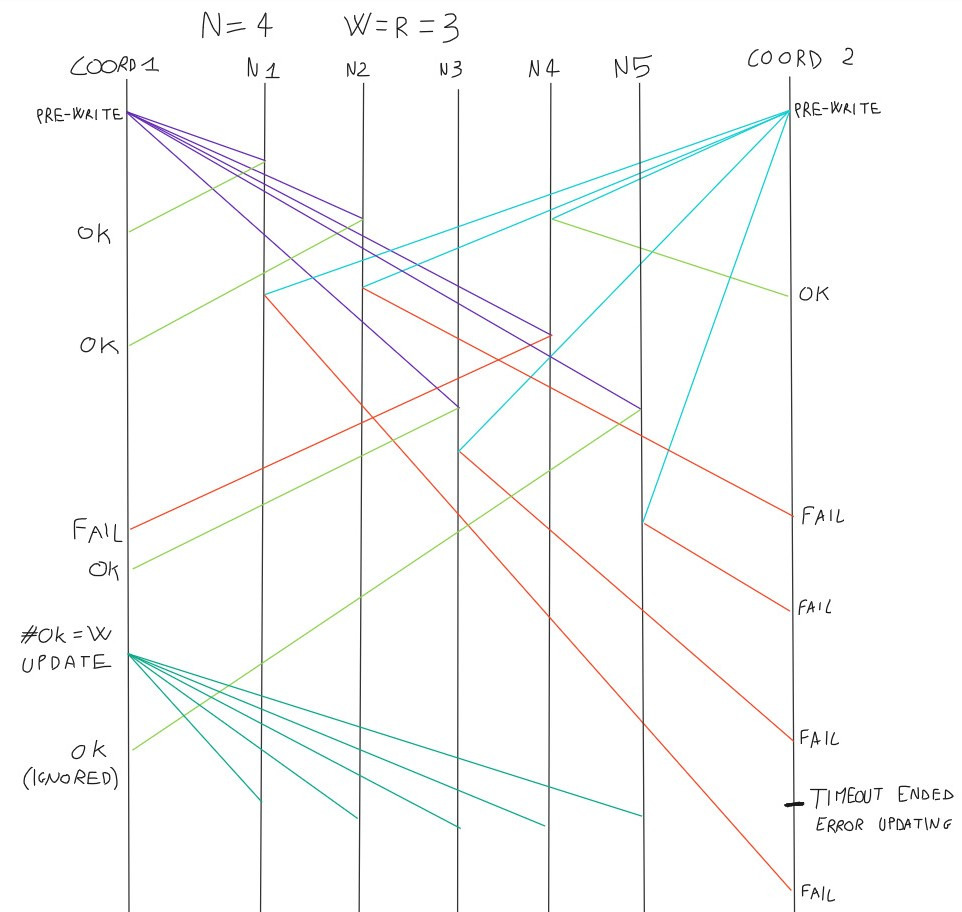
\includegraphics[width=\columnwidth]{update timeline.jpg}
        \caption{Two concurrent updates}
    \end{figure}
    
    \subsection{Get}
    Getting the value associated to a key must satisfy sequential consistency. To satisfy this requirement, we decided that not all operations must succeed, and some may fail.

    When a get operation is called, the request is forwarded, as before, to a random node that we call the coordinator. The coordinator asks to the nodes responsible for the key, calculated in the same way as before, the value they're currently storing, along with the version and the pre-write status.

    The coordinator then waits for responses until a timeout: if it is reached, we return error. As before, we wait (half+1 nodes that are responsible for the key) responses, and we call this number the read quorum R. Notice how W=R. 

    In the simplest case, let's imagine that there are no concurrent updates for the same key. Here, we simply return the value with the newest version. Remember that, for the most recent one, at least W nodes have it, so when we get R responses at least one response has the latest version (W=R $>$ 50\%).

    If there is an update in progress during a get operation, we have two cases: 
    \begin{itemize}
        \item we are in the pre-write phase, so some are in pre-write and some are not;
        \item we are in the update phase, so some have the new value while other have the old value but are in pre-write
    \end{itemize}
    The solution to keep sequential consistency is this: if we have in the responses one that has the newest version of the group and that is in pre-write, we return error. 
    
    Let's take the second case as example. Here, we know that all nodes are at least in pre-write (excluding crashed nodes, which will not recover nor respond in the middle of the operations). Some may already have received the update, but we are not sure that they are more than half N. A get operation may get two groups of responses, either we have both new values and old values in pre-write status or only old values in pre-write. If this two cases happen one after another, we could break sequential consistency by selecting only the most recent value of the R responses, because we could return first the new value and then the old one. Instead, what we need to do when we receive only old values in pre-write is return error: we know that in the system there could be a newer value, but we do not know it so we cannot return safely a response. 
    
    This could also happen where we are in the pre-write phase of the update: also here some nodes may be in the pre-write status of the most recent of the group, so here too we could return error. 
    
    \begin{figure}[H]
        \centering
        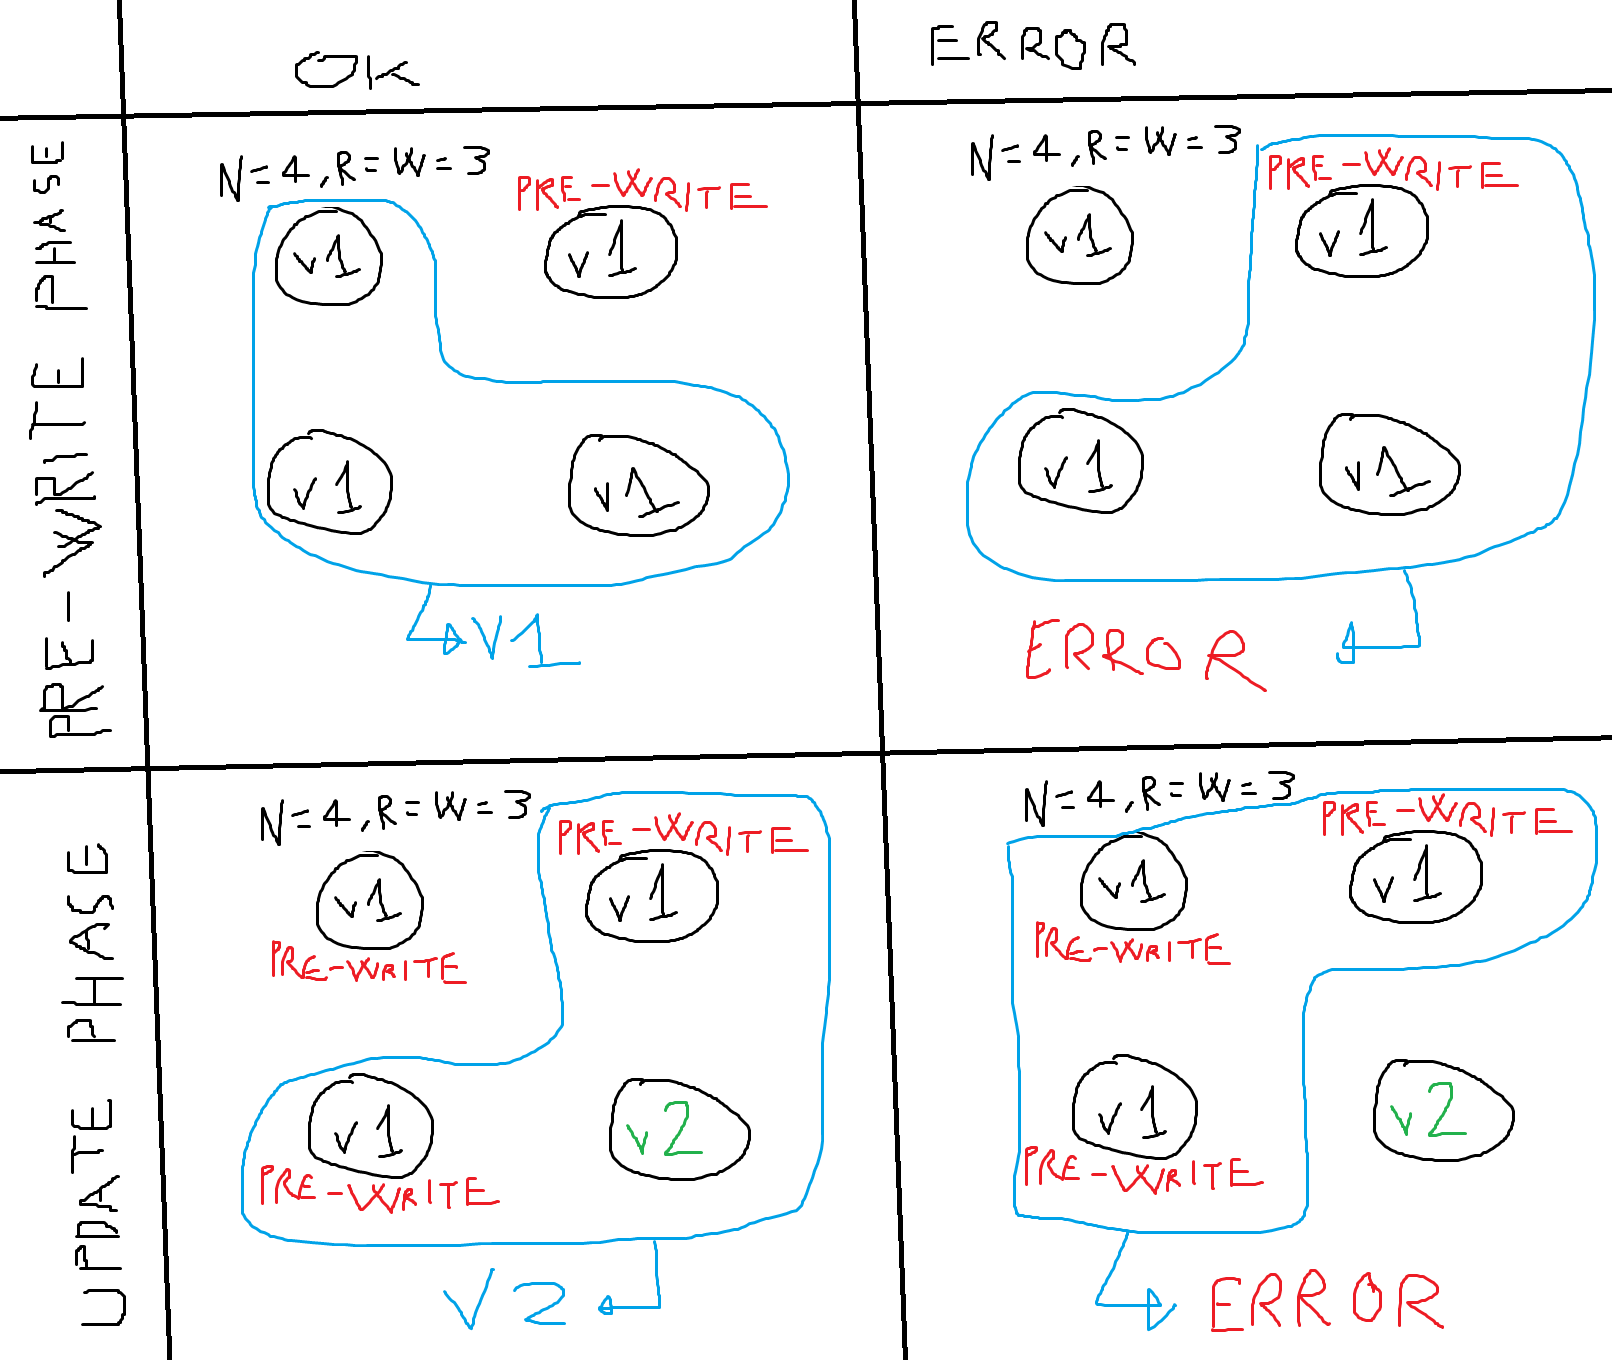
\includegraphics[width=\columnwidth]{get op.png}
        \caption{Get results}
    \end{figure}

    \pagebreak
    \section{Node Management}
    \subsection{Join}
    In the system, we have a main process that manages all nodes and clients, and it is responsible for the addition or removal of nodes. The main process may want to add a new node, with a new id, while the system is idle. Let's call both the id and the node as H. The first thing that H does is contacting another node and ask it the list of nodes in the system. If, however, H is alone, it activates itself immediately.

    Once H has received the list of nodes it searches for the node next to it in the array, let's call it H+1, and asks the list of key that H should store. It is enough to ask H+1, since it stores three types of keys: 
    \begin{itemize}
        \item keys that are kept because they are a replica in the chain of nodes, that will be passed to H; 
        \item keys greater than H-1 but smaller than H, which also will be passed to H;
        \item keys greater than H but smaller than H+1, which will not be passed.
    \end{itemize}

    So now H has the list of keys it should be responsible for. As in the get operation, H uses the function \textit{FindNodesThatKeepKey()}, calculates what key ask to what node, sends the requests for the values and stores the responses. If for a particular key we reached R values, we save the newest one to the database.

    Once we get the necessary responses for all keys or we end a timeout, H gets activated and announces itself to the others node, which will add H to the node list and analyze again all own keys with \textit{FindNodesThatKeepKey()}: if in the returned list, the node is not included it means it is no longer its responsibility, and the key gets removed from the storage.
    
    \pagebreak
    \subsection{Leave}
    The main process can ask a node to leave the system, while this is idle. Let’s call this node and its id G. Our objective with this database is making sure the get operations always respect sequential consistency. To let G leave the system, we need to be certain that by leaving the sequential consistency is respected. 

    First, G removes itself from its own node list and tells every other node to do the same. Then, it waits a timeout before continuing with the leave operation. In this way, G can finish its ongoing operations while not receiving new requests from other nodes.

    Then, the idea is to check for each key that the node which should receive it is online. If it is not, then we try to do a get operation on the key and verify two things: I can get at least R responses and the version returned is equal or greater than mine. The main problem we have is that we may be crucial to get the newest version of a key but the node that should substitute us is down, and in that case we cannot leave. When this happens, we need to void the leave operation, to avoid breaking sequential consistency.

    % Then, the idea is to do a get on all my keys and verify two thing for each key: I can get at least R responses and the version returned is equal or greater than mine. The main problem we have is that we may be crucial to get the newest version of a key but the node that should substitute us is down, and in that case we cannot leave. 

    If everything is fine, we cycle again through each key and use \textit{FindNodesThatKeepKey()}: now that G is removed from the node list, the returned array will include in the last position the node that will substitute G for that key. We collect this data and send the updates to do to the respective nodes. If the node is down, the system is sure to work fine even without this replica, since we made sure of that earlier. If the node has received in the meanwhile a newer update, the one coming from G is ignored since it has an older version that the one currently stored.

    Lastly, G deactivates itself. 
    
    \pagebreak
    \section{Crash Management}
    \subsection{Crash}
    The crash is simulated by a message from the main process. The crashed node will not process any incoming message if not related to the recovery process. A crash will not happen while an operation is ongoing, but only while the system is idle.
    
    \subsection{Recovery}
    The recovery of a node is simulated by a message from the main process. A recovery happens only while the system is idle. Let's call the node F. F can immediately return online: even if it does not hold some keys or some values have older versions, the system is able to cope with them without problems or breaking sequential consistency.
    
    The recovery message includes the node to contact to retrieve updated data since the crash. F asks this node for an updated list of all nodes in the system. F then clears the keys it is no longer responsible for, similar to how a node does after a new node joins the the system, and asks the keys it should be responsible for to the previous and next node in the list, F-1 and F+1. This is because, unless the replication factor N is 1, F is either the starting node, the ending node or somewhere in between the chain of nodes holding a key-value pair, and so it is enough to ask both the node before and after itself.

    Finally, from the lists of keys received F gets the value of the ones it is not storing yet, using the same method of asking all other nodes and deciding after R responses.

    % \pagebreak
    % \section{Demo}
    % We have made a demo to show how our program works. We start with 10 nodes [0, 10, 20, 30, 40, 50, 60, 70, 80, 90] and 2 clients. We use as replication factor N 3, so both the read and the write quorum are set to 2. We will not write the full log file here, but show only the main parts.

    % In the beginning, we initialize the clients and the nodes, without data. We then send some Update operations to fill the database. Notice how here also the decision is taken when the write quorum is reached.
    % \begin{figure}[H]
    %     \centering
    %     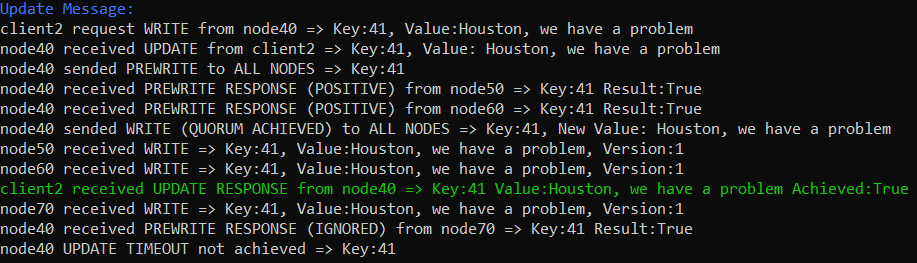
\includegraphics[width=\columnwidth]{update.png}
    %     \caption{Update key}
    % \end{figure}

    % And now that we have some data, the Get operations work. We can see how the response is given before all responses arrive.
    % \begin{figure}[H]
    %     \centering
    %     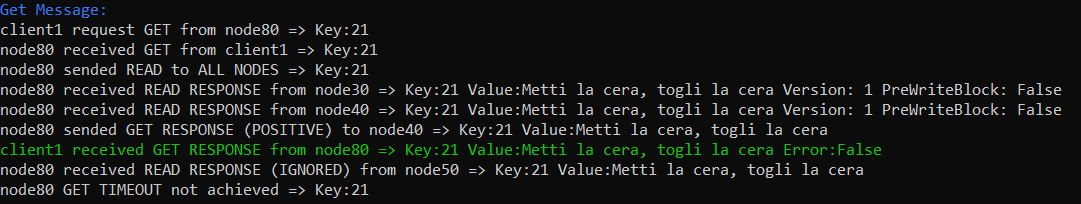
\includegraphics[width=\columnwidth]{get.png}
    %     \caption{Get key}
    % \end{figure}

    % \pagebreak
    % If we try to update the same key at the same time, at most only one succeed.
    % \begin{figure}[H]
    %     \centering
    %     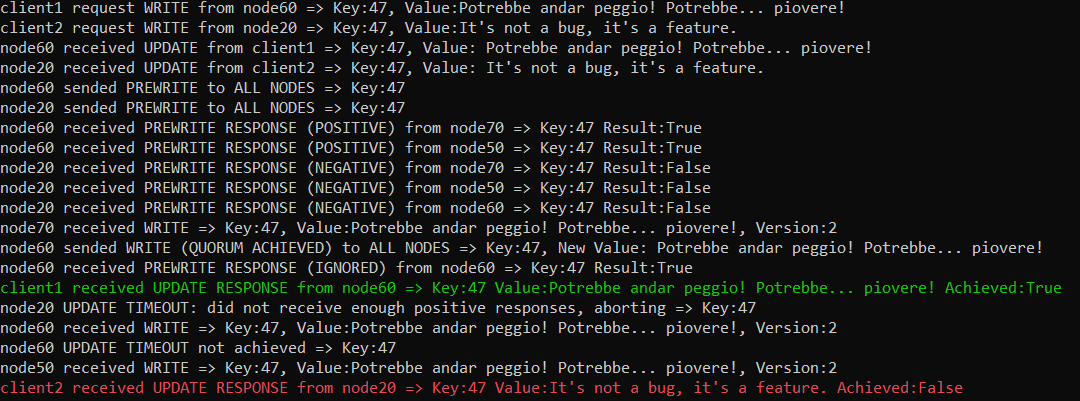
\includegraphics[width=0.85\columnwidth]{concurrent_update.png}
    %     \caption{Concurrent updates on same key}
    % \end{figure}

    % A node can join...
    % \begin{figure}[H]
    %     \centering
    %     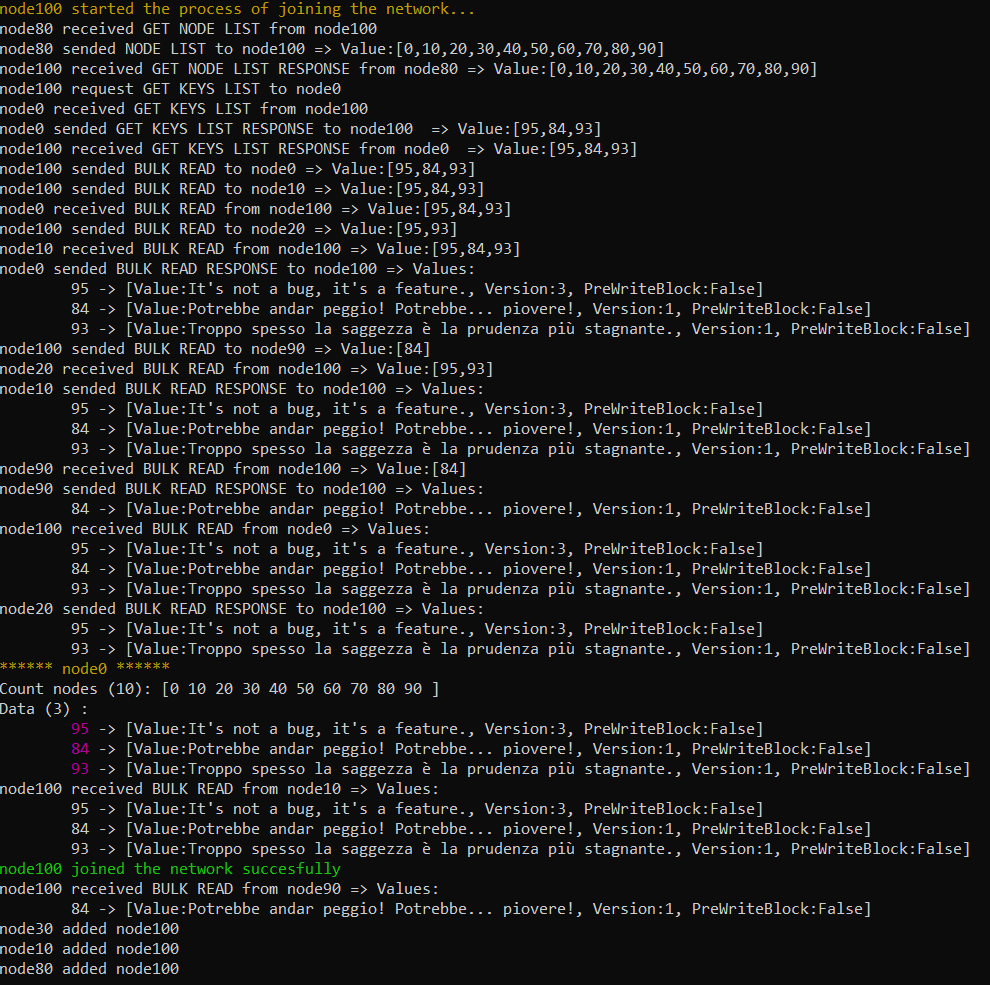
\includegraphics[width=0.85\columnwidth]{join.png}
    %     \caption{100 joins the system}
    % \end{figure}

    % \pagebreak
    % ...or leave.
    % \begin{figure}[H]
    %     \centering
    %     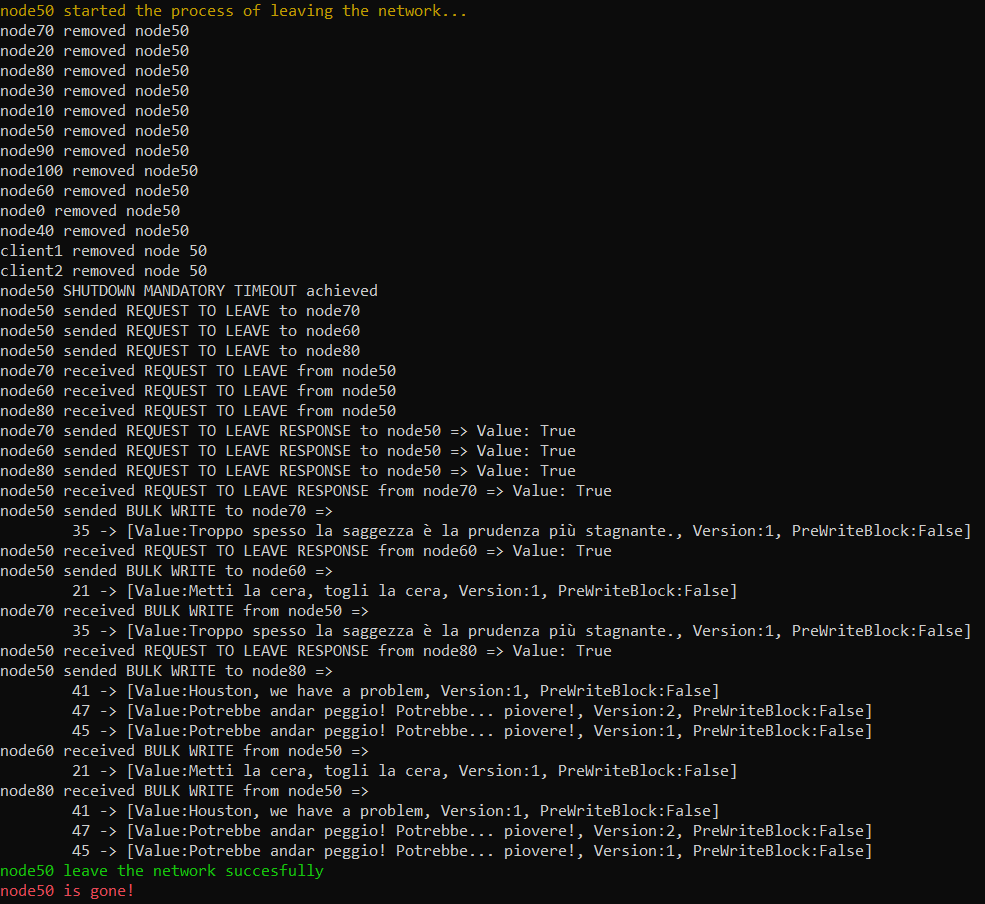
\includegraphics[width=0.9\columnwidth]{leave.png}
    %     \caption{50 leaves the system}
    % \end{figure}

    % If some nodes crash, the quorum for that key may never be reached
    % \begin{figure}[H]
    %     \centering
    %     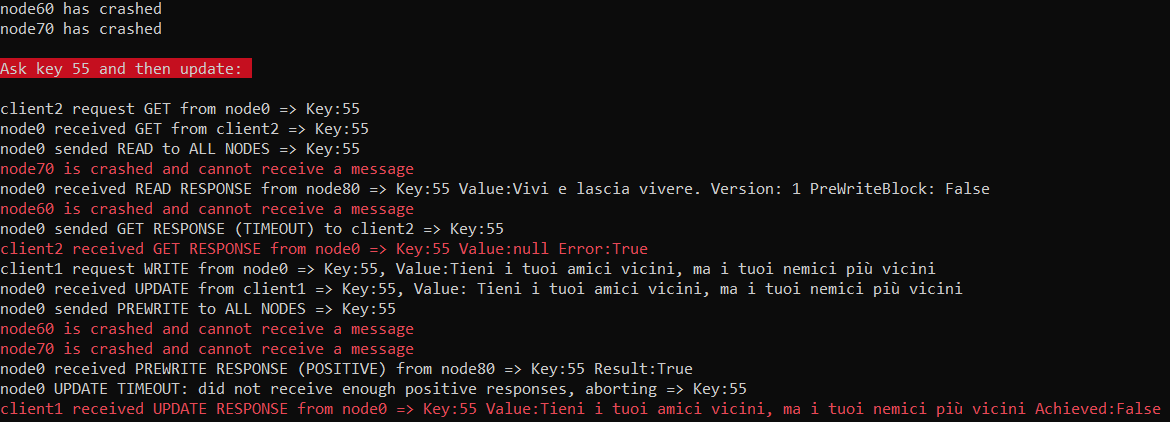
\includegraphics[width=\columnwidth]{no_quorum.png}
    %     \caption{60 and 70 crash, key 55 is unreachable}
    % \end{figure}

    % The leave may also fail because the node is too important for a key consistency.
    % \begin{figure}[H]
    %     \centering
    %     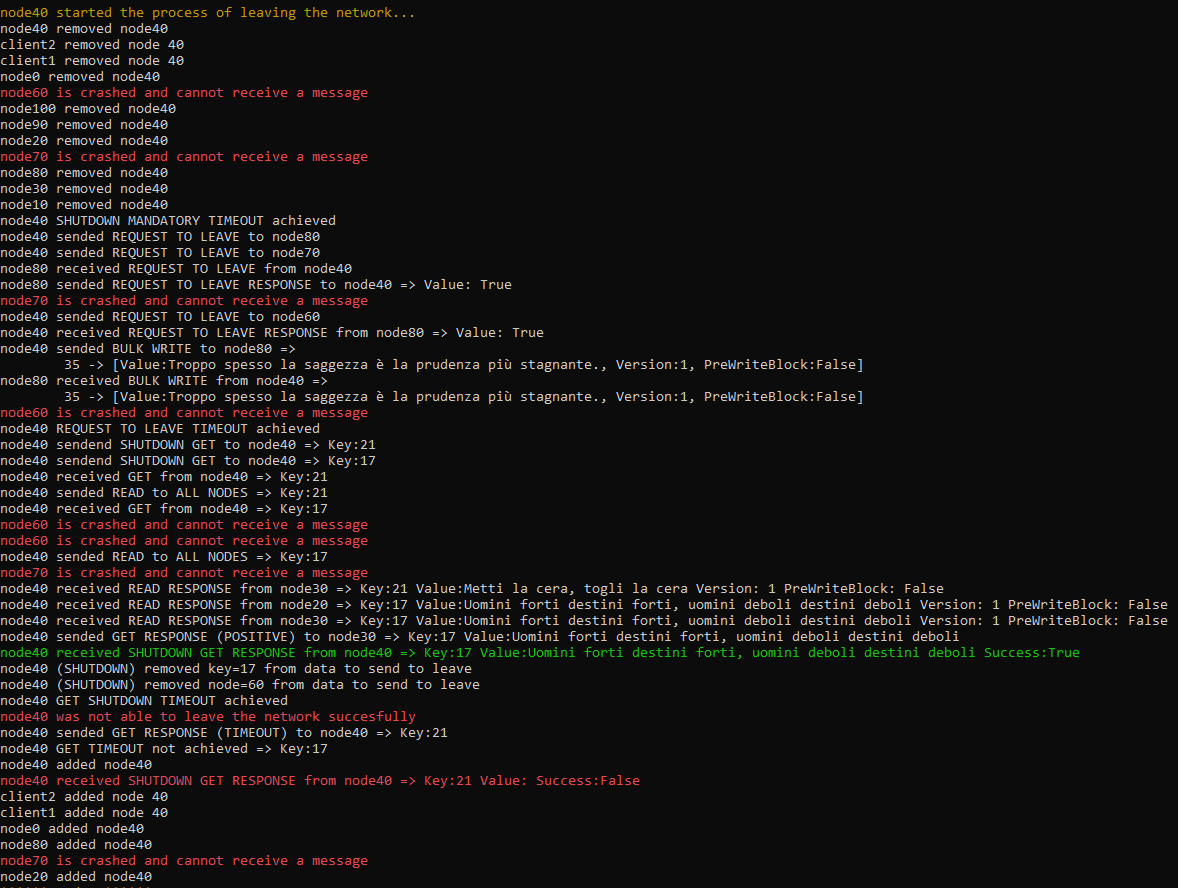
\includegraphics[width=\columnwidth]{leave_fail.png}
    %     \caption{50 leaves the system}
    % \end{figure}

    % A node can recover from a crash.
    % \begin{figure}[H]
    %     \centering
    %     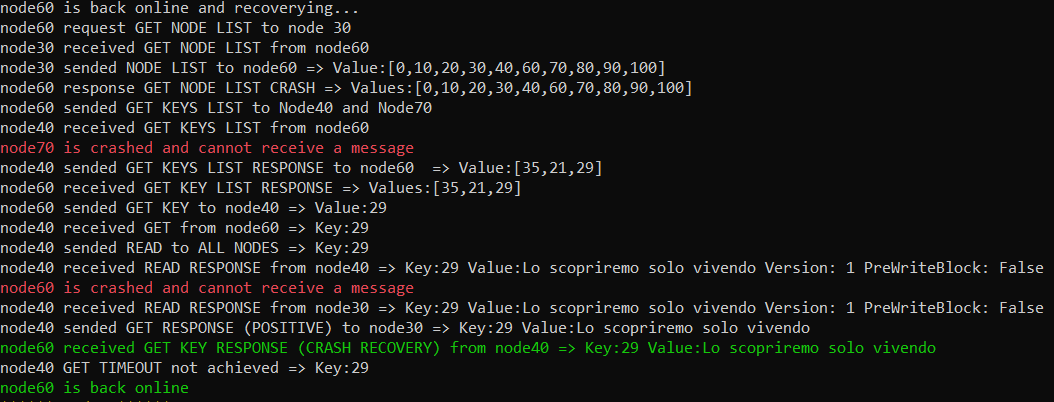
\includegraphics[width=\columnwidth]{recover.png}
    %     \caption{70 recovers}
    % \end{figure}

\end{document}
